\documentclass[convert={density=1024}]{standalone}
\usepackage{amsmath, amsthm, amsfonts}
\usepackage{tikz-cd, kotex}
\usepackage{../../preamble/quiver}
\usepackage{../../preamble/Math-operators}
\begin{document}



\end{document}

% Phase space (Classical_mechanics-1.png)
\begin{tikzpicture}
	\draw[->] (-.5,0)--(2,0) node[right]{position};
	\draw[->] (0,-.5)--(0,2) node[above]{momentum};
\end{tikzpicture}

% Kinetic energy (Classical_mechanics-2.png)
\begin{tikzpicture}
	\draw[->] (-.5,0)--(2,0) node[right]{position};
	\draw[->] (0,-.5)--(0,2) node[above]{momentum};
	\draw[red] (-.4,0)--(1.9,0);
\end{tikzpicture}

% Mechanical energy (Classical_mechanics-3.png)
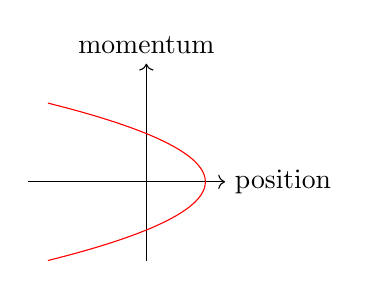
\begin{tikzpicture}
	\draw[->] (-1.5,0)--(1,0) node[right]{position};
	\draw[->] (0,-1)--(0,1.5) node[above]{momentum};
  	\draw[scale=0.5, domain=-2:2, smooth, variable=\y, red]  plot ({1.5-\y*\y}, {\y});
\end{tikzpicture}

% Harmonic oscillator (Classical_mechanics-4.png)
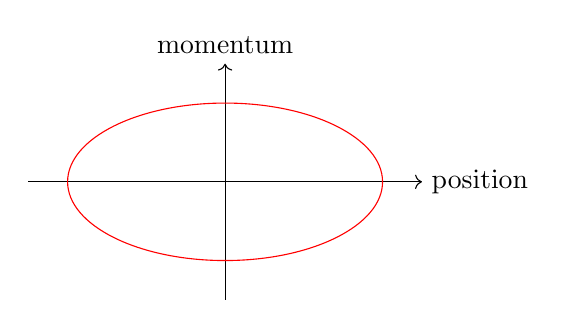
\begin{tikzpicture}
	\draw[->] (-2.5,0)--(2.5,0) node[right]{position};
	\draw[->] (0,-1.5)--(0,1.5) node[above]{momentum};
    \draw[red] (0,0) ellipse (2cm and 1cm);
\end{tikzpicture}